\documentclass[11pt,twoside,openright]{mpreport}
\usepackage[utf8]{inputenc}
\usepackage[T1]{fontenc}
\usepackage{textcomp}
\usepackage{mathptmx}
\usepackage[scaled=0.85]{helvet}
\usepackage{hyperref}
\usepackage{array}
\usepackage{ngerman}
\usepackage{glossaries}
\usepackage{color}
\usepackage{listings} \lstset{backgroundcolor=\color{lightgrey}} \lstset{language=Java}
\usepackage{wrapfig}
\usepackage{url}
\usepackage{float}
\definecolor{lightgrey}{rgb}{.9,.9,.9}

\makeindex
% makeglossaries bericht.glo

\newacronym{rup}{RUP}{Rational Unified Prozess}
\newacronym{ide}{IDE}{Integrated Development Environment}

\newacronym{api}{API}{Application Programming Interface}
\newacronym{orm}{ORM}{Object-relational mapping}

\newglossaryentry{sqlite}{
	name=SQLite,
	description={SQLite ist eine Cross Plattform Datenbankengine, welche ohne Konfiguration auskommt. Es handelt sich dabei um eine Datenbank in einer Datei},
	first={SQLite}
}

\newglossaryentry{json}{
	name={JSON},
	description={JavaScript Object Notation (JSON), ist eine Notation zur Darstellung von Objekten in Textform},
	first={JavaScript Object Notation (JSON)}
}

\newglossaryentry{enum}{
	name={Enum},
	description={Ein Enum ist ein Datentyp mit fest bestimmten Konstanten. Es kann immer nur ein Wert ausgewählt sein.}
}

\newglossaryentry{splashscreen}{
	name={Splashscreen},
	description={Eine Anzeige, die oftmals beim Start einer Applikation die Wartezeit bis zur vollständigen Initialisierung überbrückt.}
}
\newglossaryentry{csv}{
	name={CSV},
	description={Ein Dateiformat, bei welchem die Datensätze über ein Trennzeichen voneinander getrennt sind.},
	first={Comma Separated Values (CSV)}
}
\newglossaryentry{http}{
	name={HTTP},
	description={Das Hypertext Transfer Protocol (HTTP) ist ein weit verbreitetes Protokoll, um Daten und Inhalte im Web zu übertragen. In dieser Arbeit wird es in der Kommunikation mit dem Server verwendet.},
	first={Hypertext Transfer Protocol (HTTP)}
}
\newglossaryentry{junit}{
	name={JUnit Test},
	description={Java bietet die Möglichkeit integrierte Softwaretests automatisiert durchzuführen. Dies erleichtert die Arbeit enorm und unterstützt ein Entwicklungsteam, eine möglichst hohe Testabdeckung zu erarbeiten},
	first={Java Unit Test (JUnit)}
}

\newglossaryentry{chronofunk}{
	name={Chronofunk},
	description={Die Motorradfahrer, welche im Rennfeld verteilt mitfahren und die Positionen der Ausreissergruppen per Funk an den RadioTour Speaker übermitteln}
}

\makeglossaries

\begin{document}
\setlength{\oddsidemargin}{50mm}
	\title{Android Applikation RadioTour}
	\author{Florian Bentele \& Daniel Stucki}
 	\maketitle

\chapter*{Abstract}


Bisher mussten bei Radrennen Motorradfahrer die Nummern der Fahrer, welche aus dem Feld ausgerissen sind, einem \textit{RadioTour Speaker} melden. Dieser meldet dann die Ausreisser jeweils per Funk an die Mannschaftsleiter weiter. Bei den meisten Radrennen notieren die \textit{RadioTour Speaker} die erhaltenen Informationen auf einem Notizbuch, bevor sie die Fahrernummern weitergeben. An der Tour de Suisse arbeitet man seit einigen Jahren mit einer Tablet-PC Web Applikation zur elektronischen Erfassung der Renninformationen.
\\
Die im Rahmen dieser Studienarbeit realisierte \textit{RadioTour} Android Tablet Applikation ersetzt und erweitert die "`in die Jahre gekommene"' webbasierte Tablet-PC Anwendung. Die neue native \textit{RadioTour} Android Anwendung bietet eine einfachere Touchscreen Bedienung, verbesserte Importfunktionen sowie neue Features wie beispielsweise Live-Marschtabellen und Streckenkilometerbestimmung aus den lokalen GPS-Daten. Verbessert wurde auch die Kommunikation mit der TourLive Webseite via JSON zur unmittelbaren Veröffentlichung der aktuellen Rennsituationen. Die Anwendung ist bewusst für Android Honeycomb \& Ice Cream Sandwich und für die  spezifische Hardware-Plattform eines Samsung Galaxy Tab 10.1 entwickelt worden, da das System zusammen mit der Hardware-Plattform zur Verfügung gestellt wird.
\\
Für die Entwicklung der Applikation kommt die Java IDE Eclipse (Version Indigo) zur Anwendung. Die Datenpersistierung auf dem Tablet wird mithilfe der ORMLite Library (Version 4.39) in einer SQLite Datenbank umgesetzt.
\\
Der Release 1 wurde an der Berner Rundfahrt 2012 getestet. Die dort gewonnenen Erkenntnisse wurden im Release 2 berücksichtigt, so dass nun ein System vorliegt, welches die Grundanforderungen erfüllt. Letzte, kleinere Anpassungen wird der Industriepartner im Rahmen der Systemübernahme vornehmen. Die neue RadioTour Anwendung wird voraussichtlich bei der Tour de Suisse 2012 zum Einsatz kommen.

\chapter*{Aufgabenstellung}

\begin{tabular}{ll}
Studiengang: & Informatik (I)\\
Semester: & FS 2012 (21.02.2012-01.06.2012)\\
Institut: & ITA: Internet-Technologien und Anwendungen\\
Gruppe: & Florian Bentele, Daniel Stucki\\
Verantwortlicher: & Dr. Prof. Peter Heinzmann, pheinzma@hsr.ch\\
Industriepartner: & cnlab AG, Lukas Frey, lukas.frey@cnlab.ch

\end{tabular}

\section*{Ausgangslage}
Bei Radrennen erfasst der so genannte \textit{RadioTour Speaker} Informationen zur Rennsituation, welche ihm von Motorradfahrern per Funk geliefert werden. Gegenwärtig legt der \textit{RadioTour Speaker} mit Hilfe einer TabletPC Web-Anwendung per Click auf die erhaltenen Fahrernummern die Zusammensetzung der Gruppen fest. Er tippt auch die Zeitabstände zwischen den Gruppen ein. Die \textit{RadioTour} Anwendung  visualisiert die Fahrergruppen und liefert Detailinformationen zu den Fahrern (z.B. Namen, Team, virtueller Rang). Veränderungen in den Fahrergruppen können per Drag-and-Drop nachgeführt werden. Die mit der \textit{RadioTour} Anwendung erfassten Rennsituationen werden per Mobilfunknetz zu einem Webserver gesendet, wo sie weiteren Anwendungen, z.B. Live Webinformationen zur Verfügung stehen.

\section*{Ziel}
Die aus dem Jahre 2006 stammende Notebook Web Applikation soll nun dahingehend überarbeitet und erweitert werden, dass man sie auf Android-Tablets oder iPads betreiben kann.
\\
Das Produkt wird spezifisch auf ein Gerät und nicht plattformübergreifend entwickelt. Die Verbindung zum Server wird in der Arbeit definiert, jedoch werden keine serverseitigen Entwicklungen erarbeitet.
\\
Die Mehrsprachigkeit wird nach Android Standards implementiert \footnote{Android Internationalisierung, \url{http://developer.android.com/guide/topics/resources/localization.html}}. Eine Übersetzung ist jedoch nicht Teil der Arbeit.
\newpage

\section*{Teilaufgaben}
\begin{itemize}
\item Analyse der existierenden \textit{RadioTour} und TourLive-Anwendungen
\begin{itemize}
\item Tour de Suisse Dokumente
\item Alte \textit{RadioTour} Anwendung\\
\url{http://gps.cnlab.ch/tablet/}\\
user: ba\_tourlive\\
password: access4tl
\item TourLive-System (GPS Positions- und Bilderfassungssysteme, Webanwendung)
\item Kommunikation \textit{RadioTour} – TourLive-Webanwendung
\item Vergleich mit Systemen anderer Radrennen 
\end{itemize}

\item Festlegung der Funktionalität der neuen Tablet-Anwendung (Requirements Engineering)
\begin{itemize}
\item Studium der Geschäftsprozesse (Renninformationen, Rennverlauf)
\item Austesten von Teilfunktionen (Android-Tablet Programmierung, GPS-Positionserfassung, Usability Experimente)
\item Erweiterte Funktionen (z.B. Erfassung der Streckenkilometer, Integration von Marschtabellen)
\item Auswahl der Hardware-Plattform
\item Spezifikation
\end{itemize}

\item Design
\begin{itemize}
\item Benutzerschnittstelle
\item Kommunikation mit TourLive Aufnahmesystemen (Weitergabe der Daten an Datenserver)
\item \textit{RadioTour} Anwendung
\end{itemize}

\item Realisierung
\begin{itemize}
\item Prototypen
\item Anpassungen
\item Friendly User Test Version (Beta-Release)
\item Feldtest an einem Radrennen
\item Übergabe an cnlab
\end{itemize}

\item Dokumentation
\begin{itemize}
\item Gemäss Anforderungen Industriepartner (das System soll vom Industriepartner betrieben und erweitert werden können)
\item Bericht gemäss HSR / Heinzmann Richtlinien
\end{itemize}
\end{itemize}

Diese Aufgabenstellung wird genehmigt vom Betreuer
\\
\\

\begin{tabular}{p{3cm}p{4cm}}
\hline
Ort / Datum & P. Heinzmann
\end{tabular}

\section*{Erklärung zur Urheberschaft\footnote{Diese Erklärung basiert auf der Muster-Erklärung in den Richtlinien der HSR zur Durchführung von Projekt-, Studien-, Diplom- oder Bachelorarbeiten vom 16. Februar 2009.}}
Die vorliegende Arbeit basiert auf Ideen, Arbeitsleistungen, Hilfestellungen und Beiträgen gemäss folgender Aufstellung:
\\

\begin{tabular}{|m{5cm}|m{3.7cm}|m{3cm}|}
\hline
Gegenstand, Leistung & Person & Funktion \\[5pt]\hline\hline
Kapitel 3, 4, 5 und Anhänge & Daniel Stucki & Autor der Arbeit\\[5pt]\hline
Kapitel 1, 2, 5, 6 und Anhänge & Florian Bentele & Autor der Arbeit\\[5pt]\hline
Korrektur & Heinrich Stucki & Lektorat \\[5pt]\hline
Korrektur & Doris Bentele & Lektorat \\[5pt]\hline
Korrektur & Ursina Bentele & Lektorat \\[5pt]\hline
Idee, Aufgabenstellung, allgemeines Pflichtenheft, Betreuung während der Arbeit & Prof. Dr. P. Heinzmann & Verantwortlicher Professor \\[5pt]\hline
Industriepartner und Ansprechperson & Lukas Frey & cnlab AG \\[5pt]\hline
\end{tabular}
\\
\\

Ich erkläre hiermit,
\begin{itemize}
\item dass ich die vorliegende Arbeit gemäss obiger Zusammenstellung selber und ohne weitere fremde Hilfe durchgeführt habe,
\item dass ich sämtliche verwendeten Quellen erwähnt und gemäss gängigen wissenschaftlichen Zitierregeln korrekt angegeben habe.
\end{itemize}

Rapperswil, 29. Mai 2012
\\
\\

\begin{tabular}{p{5cm}p{5cm}}
\hline

Florian Bentele & Daniel Stucki
\end{tabular}

\newpage

\section*{Vereinbarung zur Verwendung und Weiterentwicklung der Arbeit\footnote{Diese Vereinbarung basiert auf den Muster-Vereinbarungen in den Richtlinien der HSR zur Durchführung von Projekt-, Studien-, Diplom- oder Bachelorarbeiten vom 16. Februar 2009.}}

\textbf{1. Gegenstand der Vereinbarung}
\\
Mit dieser Vereinbarung werden die Rechte über die Verwendung und die Weiterentwicklung der Ergebnisse der \thesistype \ "`\thesistitle "'  von \thesisauthora \ und \thesisauthorb \ unter der Betreuung von \professor \ (für die Arbeit verantwortlicher Professor) geregelt.
\\

\textbf{2. Urheberrecht}
\\
Die Urheberrechte stehen der Studentin / dem Student zu.
\\

\textbf{3. Verwendung}
\\
Die Ergebnisse der Arbeit dürfen sowohl von allen an der Arbeit beteiligten Parteien, d.h. von den Studenten, welche die Arbeit verfasst haben, vom verantwortlichen Professor sowie vom Industriepartner verwendet und weiter entwickelt werden. Die Namensnennung der beteiligten Parteien ist bei der Weiterverwendung erwünscht, aber nicht Pflicht.
\\

\begin{tabular}{p{5cm}p{1cm}p{6cm}}
Rapperswil, den  & & \\[30pt]
\hline
 & & \thesisauthora \\[10pt]
Rapperswil, den  & & \\[30pt]
\hline
 & & \thesisauthorb \\[10pt]
Rapperswil, den  & & \\[30pt]
\hline
 & & \professor \\[10pt]
Rapperswil, den  & & \\[30pt]
\hline
 & & Industriepartner, Lukas Frey, cnlab AG \\
\end{tabular}

\chapter*{Management Summary}

\section*{Ausgangslage}
An der Tour de Suisse fahren ca. 200 Radrennfahrer in Tagesetappen durch die ganze Schweiz. Dabei werden Sie von diversen Motorfahrzeugen begleitet. Im Radfahrer-Feld fährt ebenfalls der \textit{RadioTour Speaker} mit. Seine Funktion besteht darin, Live Informationen des Rennens zu erfassen und an den Server der cnlab AG weiterzuleiten.  Die Übertragung der Daten vom Gerät zum Server geschieht über das Mobilfunknetz 3G.

\subsection*{Live Informationen}
Während dem Rennen werden aus verschiedenen Quellen Informationen gesammelt. Zum einen sind dies Veränderungen im Rennfeld, zum anderen Wertungen, welche die Fahrer erreichen können, so z.B. einen Bergsprint. Diese Daten werden vom \textit{RadioTour Speaker} manuell erfasst.
\\
Wenn sich ein Rennfahrer vom Feld ablöst und einen Vorsprung erarbeitet, wird dieser von einem Motorradfahrer verfolgt. Diese Änderung wird dann sofort per Funk an den \textit{RadioTour Speaker} übermittelt.

\subsection*{Äussere Bedingungen}
Bei Live Sport Events wie der Tour de Suisse ist die Erfassung von Echtzeitdaten, aus technischer Sicht, eine Herausforderung. Sowohl das Alpine Gebirge, wo die Mobilfunkverbindungen und GPS Informationen nicht immer gewährleistet sind, als auch die ständige Vibration der Fahrzeuge stellen erschwerende Rahmenbedingungen dar.
\\
Die Unterbrüche der Verbindung werden überbrückt, indem die Änderungen gesammelt und periodisch an den Server gesendet werde. Alle Änderungen werden als Paket in eine Warteschlange eingetragen. Ist eine sofortige Übertragen nicht möglich, wird es später wieder versucht.


\section*{Vorgehensweise}
In der vorliegenden Studienarbeit kommt das Vorgehensmodell zur Softwareentwicklung von \gls{rup} zur Anwendung. Das Projekt wird in die folgenden vier Phasen aufgeteilt:

\begin{enumerate}
\item Inception
\item Elaboration
\item Construction
\item Transition
\end{enumerate}

In jeder dieser Phasen werden die Arbeitsschritte nach \gls{rup} durchgeführt, je nach dem in mehreren Iterationen, wie es bei dieser Arbeit in der Phase \textit{Construction} vorkommt.\footnote{Wikipedia, Rational Unified Process,  \url{http://de.wikipedia.org/wiki/Rational_Unified_Proces}, aufgerufen am 20.05.2012.}
\\
Die Erfassung der Anforderungen, der Entscheid zur Entwicklung auf einem Android Gerät sowie die Evaluation eines geeigneten Tablets bilden zusammen die Startphase des Projekts. Die Anforderungskriterien an das Tablet wurden in einer Sitzung zusammen mit Herrn Dr. Prof. Peter Heinzmann, dem Betreuer der Arbeit, diskutiert und genehmigt.
\\
Im weiteren Verlauf der Arbeit wurden die Anforderungen und die UseCases definiert. Daraus entstand dann die Domainlogik und parallel dazu ein erster Prototyp des UserInterface. Insbesondere die Benutzerschnittstelle entstand in mehreren Iterationen, da eine gute Bedienung für den Erfolg des Produktes entscheidend ist, dies jedoch erst bei der realen Anwendung geprüft werden kann.

\section*{Ergebnisse}
Die \textit{RadioTour} Android Applikation beinhaltet die festgelegten Anforderungen. Die Fahrerlisten und die offiziellen Zeitmessungen können via USB oder aus dem Internet importiert werden. Die Gruppen lassen sich dynamisch verändern und die Rennsituation wird an den Server übermittelt. Ein Testlauf mit dem ersten Prototypen hat klar aufgezeigt, dass diese Anwendung eine Verbesserung in der Bedienung bringt. Dabei entstehen keine Einbussen in der Funktionalität. Die Applikation ist damit für den Einsatz an der Tour de Suisse bereit.


\section*{Ausblick}
Für den erfolgreichen Einsatz an der Tour de Suisse ist ein Feldtest, insbesondere um die Serververbindung zu testen, notwendig.
\\
Nach der Tour de Suisse sind die Eindrücke und das Feedback des \textit{RadioTour Speakers} aufzunehmen, damit die Applikation weiter verbessert werden kann.

\tableofcontents

\chapter{Einleitung}

Im folgenden Abschnitt werden die aus technischer Sicht relevanten Aspekte genauer analysiert. Zu Beginn wird das Aufgabenumfeld in einem weiteren Sinne betrachtet, und die Kernelemente der Applikation aufgezeigt. Danach wird auf die Analyse und die Realisierung eingegangen.
\\
Der Hauptteil richtet sich vor allem an Personen, die bereits Hintergrundwissen zu Android vorweisen, sowie für Entwickler, die an der Weiterentwicklung des Produktes interessiert sind.

\section{BigPicture}
Zur Übersicht wird das Umfeld der Applikation in einem BigPicture zusammengefasst. Es ermöglicht die Darstellung der äusseren Einflussfaktoren sowie die Abgrenzung des Systems zu definieren.
\\
Die schematische Darstellung zeigt im wesentlichen die drei Hauptakteure auf. Zum einen sind dies die Motorradfahrer, welche die Radrennfahrer begleiten und Veränderungen in Echtzeit per Funk übermitteln. Diese Informationen kommen in kurzen Abständen und müssen sofort erfasst werden. Im UserInterface wird dafür eine Lösung verwendet, bei der mehrere Radrennfahrer gleichzeitig eingetragen werden können.
\\
Eine weitere Rolle spielt der \textit{RadioTour Speaker} mit dem Android Tablet. Er fasst die Informationen zusammen und wertet diese bereits bei der Eingabe auf dem Gerät aus. Im Tablet werden auch Daten wie z.B. die Durchschnittsgeschwindigkeit und die aktuelle Rennzeit angezeigt.
\\
Der dritte Akteur bildet der Server der cnlab AG, welcher direkt mit der Applikation kommuniziert. Ausgetauscht werden die Veränderungen im Feld sowie Rückstände von der Spitze. Weiter können Ereignisse wie z.B. eine Verletzung oder ein defektes Fahrrad aufgezeichnet werden. Die Daten werden dann weiter auf der Webseite der \textit{TourLive} aufbereitet und publiziert. Nicht nur für die Beteiligten im Team, sondern auch für Fans sind diese Angaben von grossem Interesse, da die Daten vor den offiziellen Zeitmessungen bereits einen Einblick in das Schlussklassement geben.

\newpage

\begin{figure}[h!]
\caption{Das Aufgabenumfeld in einem BigPicture zusammengefasst}
\centering
\includegraphics[scale=0.7]{05bericht/images/bigpicture.png}
\end{figure}

\newpage

\section{Kernelemente}
Das Produkt dieser Arbeit ist es, die Tabletanwendung für den \textit{RadioTour Speaker} zu entwickeln. Der Hauptfokus liegt dabei auf der Erfassung der Rennsituation und die sichere Übertragung an den Server. In der Abbildung \ref{fig:closepicture} steht die Applikation im Mittelpunkt und zeigt die \gls{http} Schnittstelle zum TourLive Server. Die Positionsdaten werden von den GPS Satelliten empfangen und die Datenpersistierung basiert auf einer \gls{sqlite} Datenbank. In der Applikation ist die Hauptansicht für die Situation während einem Rennen zu sehen.
\\

\begin{figure}[h!]
\caption{Die genaue Betrachtung der Aufgaben der Applikation}
\label{fig:closepicture}
\centering
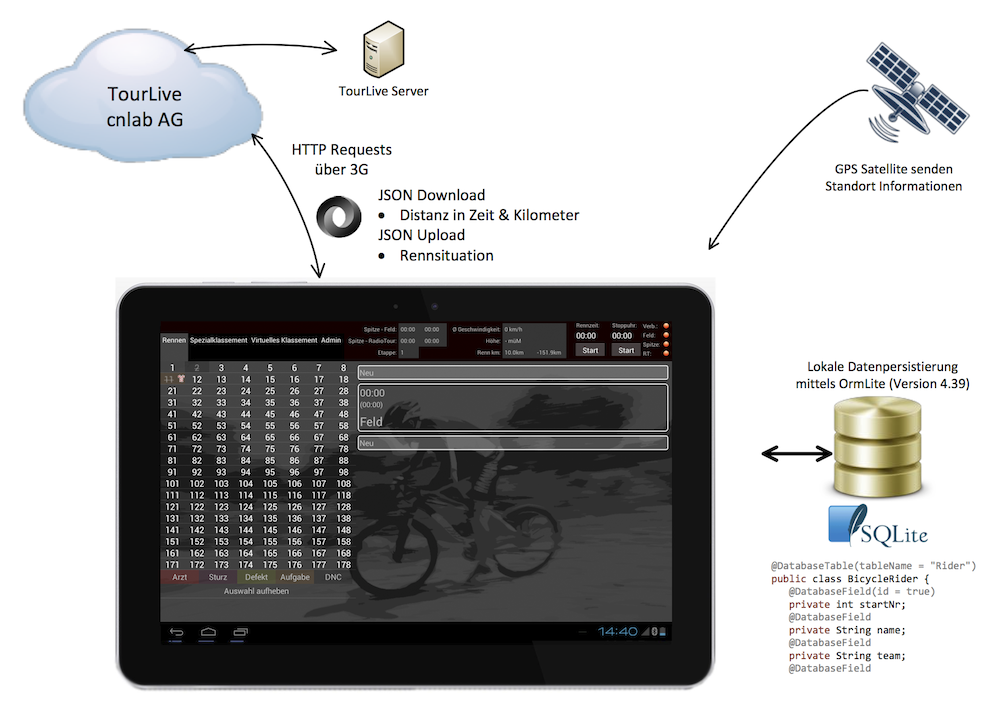
\includegraphics[scale=0.8]{05bericht/images/closepicture.png}
\end{figure}

\chapter{Analyse}
Die Analyse untersucht die bestehende Web Applikation und fasst die Anforderungen zusammen. Danach wird die Plattform und die passende Hardware dazu evaluiert und in Form einer Kaufempfehlung an die cnlab AG weitergeleitet. Es werden die verwendeten Technologien sowie ein kurzer Exkurs zu anderen Lösungen angesprochen.

\section{Requirements}
\label{sec:requirements}
Die Anforderungen an die \textit{RadioTour} Applikation ergeben sich aus den Features der bisherigen Web Applikation und den Verbesserungsvorschlägen des \textit{RadioTour} Speakers. Im Anhang \ref{ref:usecases} sind sämtliche UseCases der bisherigen Applikation aufgeführt. Im folgenden Abschnitt werden die Funktionen, welche in diesem Projekt implementiert sind, aufgeführt.

\subsection{Funktionale Anforderungen}
Die funktionalen Anforderungen sind in drei Prioritätsstufen eingeteilt:

\textbf{zwingende Anforderungen (must)}
\begin{itemize}
\item Fahrerliste, Etappen und Marschtabellen importieren
\item Fahrer ansehen, sortieren und bearbeiten
\item Gruppen bilden und Rückstand angeben
\item Gruppen auflösen
\item Events für Fahrer erfassen (Sturz, Arzt, Aufgabe)
\item Rennsituation an den Server übermitteln
\item Spezialklassemente und Wertungen erstellen und Fahrer zuweisen
\item Maillots erfassen und bearbeiten
\item Persistierung der Daten auf dem Gerät

\end{itemize}


\textbf{optionale Anforderungen (can)}
\begin{itemize}
\item Aktuelle Rennkilometer und Rennzeit anzeigen
\item Stoppuhr
\item Aktuelle Position durch GPS bestimmen
\item Events für Fahrer an den Server übermitteln
\end{itemize}


\textbf{wünschenswerte Anforderungen (nice to have)}
\begin{itemize}
\item Aktuelle Position des \textit{RadioTour Speakers} in der Marschtabelle anzeigen
\item \gls{splashscreen} beim Start der Applikation
\end{itemize}

\subsection{Nicht funktionale Anforderungen}
Im Umfeld eines Live Sport Events spielen neben den funktionalen Anforderungen an ein Software Produkt auch nicht funktionale Anforderungen eine wichtige Rolle. So muss z.B. das UserInterface Fehler bei der Eingabe tolerieren bzw. korrigierbar machen. Die Bedienung muss flüssig verlaufen und zu jedem Zeitpunkt muss der Status der Applikation sichtbar sein. Die für \textit{RadioTour} relevanten nicht funktionalen Anforderungen sind im Folgenden aufgelistet.

\begin{itemize}
\item Mobilfunkverbindung ist nicht immer gewährleistet, keine Daten dürfen dadurch verloren gehen
\item Informationen müssen auch bei direktem Sonnenlicht gut lesbar sein
\item Angenehme, flüssige und selbsterklärende Bedienung der Applikation
\end{itemize}

Weitere nicht funktionale Anforderungen beziehen sich auch auf die Hardware an sich und sind im Kapitel \ref{kap:kaufempfehlung} bereits aufgeführt.

\section{Evaluation und Kaufempfehlung}
\label{kap:kaufempfehlung}
Die Evaluation der Zielplattform war ein wichtiger Faktor für die weitere Entwicklung der Arbeit. Aus diesem Grund stand diese ganz zu Beginn der Arbeit an. Zur Auswahl standen die beiden marktführenden Betriebssysteme Android (Google) und iOS (Apple). Als Grundlage für die Evaluation dienten die folgenden Kriterien:
\begin{itemize}
\item Vorkenntnisse der Programmiersprachen Java bzw. Objective-C
\item Möglichkeiten zum UserInterface Design
\item Programmierumgebung, \gls{ide}
\item Mögliche Vertriebskanäle der Applikation
\item Nutzbarkeit von externen Geräten und Schnittstellen
\item Vielfalt von Informationsquellen im Internet
\end{itemize}
Die Kriterien werden in einer Nutzwertanalyse gewichtet und bewertet. Insbesondere die Vorkenntnisse in Java sind  ausschlaggebend für den Entscheid, die Applikation für die Androidplattform zu entwickeln. Dieser Entscheid ist in Absprache mit Herrn Heinzmann getroffen worden. Die gesamte Liste der Kriterien mit der jeweiligen Gewichtung sowie eine ausführliche Erläuterung befinden sich im Anhang \ref{ref:kriterien}.
\\

Für die Auswahl eines geeigneten Tablets wird im nächsten Schritt ein Kriterienkatalog definiert mit zwingenden und optionalen Kriterien für das Gerät. Die zwingenden Kriterien beinhalten:
\begin{itemize}
\item Android Betriebssystem, gemäss Evaluation
\item USB Anschluss für den Import der Fahrerliste am Renntag, optional auch mit Adapter möglich
\item Mobilfunktnetz 3G für die Kommunikation mit dem Server
\item GPS für die Lokalisierung
\item Stromversorgung durch 12V (Auto) Adapter möglich
\end{itemize}
Zu den optionalen Kriterien gehören die Akkulaufzeit, falls die Stromversorgung unterbrochen wird, sowie ein grosszügiger Bildschirm für die Bedienung mit dem Finger oder mithilfe eines Stifts.
\\

Als Sieger und somit auch als Kaufempfehlung an die \textit{cnlab AG} geht das Lenovo ThinkPad Tablet. Dieses Gerät erfüllt alle Kriterien und überzeugt in der Vielfalt der Anschlüsse. Die Kaufempfehlung mit weiteren Erläuterungen ist ebenfalls im Anhang \ref{ref:kaufempfehlung} zu finden.
\\

Im Verlauf der Arbeit ist ein Defekt an der Micro USB Buchse entstanden. Dieser Anschluss wird für die Entwicklung auf dem Gerät dringend benötigt. Für die weitere Entwicklung ist ein Ersatzgerät angeschafft worden. Dabei handelt es sich um das Galaxy Nexus Tab 10.1\footnote{Galaxy Nexus Tab 10.1, \url{http://www.samsung.com/ch/consumer/mobile-phone/tablets/tablets/GT-P7500UWDITV}, Aufgerufen am 23.05.2012.}

\section{Technologien}
\subsection{Android}
Die native Programmiersprache für das Android Betriebssystem ist Java. Die Programmierung in Java bringt den Vorteil, dass auf die gesamte \gls{api} von Android zugegriffen werden kann. Weiter sind die Geräte genau dafür ausgelegt und eine optimale Performance kann erreicht werden. Sämtliche Komponenten dieser Arbeit sind in Java geschrieben. Für die Persistierung der Daten auf dem Tablet wird eine \gls{sqlite} Datenbank verwendet.

\subsection{Externe Libraries}
Android beinhaltet bereits ein umfangreiches Framework zur Entwicklung. Deshalb nutzt die \textit{RadioTour} Applikation folgende zwei externe Libraries:
\\

\textit{ORMLite}\footnote{ORMLite, \url{http://ormlite.com/}, aufgerufen am 23.05.2012} ist eine OpenSource Java Library, welche das \gls{orm} übernimmt. ORMLite bietet eine speziell auf Android angepasste Distribution. Um eine Klasse mit ihren Feldern zur Persistierung zu markieren, werden Java Annotationen verwendet. Aus diesen Annotationen erstellt ORMLite die Datenbank. Darüber hinaus werden mit ORMLite alle Zugriffe auf die \gls{sqlite} Datenbank ausgeführt. In dieser Arbeit wird die ORMLite Version 4.39 verwendet.
\\

\textit{Robotium}\footnote{Robotium, \url{http://code.google.com/p/robotium/}, aufgerufen am 30.05.2012.} ist ein Test Framework, welches unter der Apache License 2.0 veröffentlicht und zur freien Nutzung angeboten wird. Robotium untersützt das Testen der Applikation mithilfe von UI Aktionen. In dieser Arbeit wird die Version 3.2.1 von Robotium verwendet.


\subsection{Entwicklungsumgebung}
Die von Android empfohlene Entwicklungsumgebung ist Eclipse\footnote{Eclipse, \url{http://eclipse.org/}, aufgerufen am 11.05.2012.} mit einem Plugin zur Entwicklung von Android Applikationen. Auf der Entwicklerseite von Android steht dazu folgendes:
\begin{quote}
\textit{Android Development Tools (ADT) is a plugin for the Eclipse IDE that is designed to give you a powerful, integrated environment in which to build Android applications.}\footnote{Android Plugin für Eclipse, \url{http://developer.android.com/sdk/eclipse-adt.html}, aufgerufen am 01.05.2012.}
\end{quote}
Eclipse ist eine weit verbreitete \gls{ide} und wird aktiv weiter entwickelt. Mit dem Plugin zusammen bildet sie eine solide Grundlage für dieses Projekt.
\\

Damit die Android Applikation direkt auf dem Computer getestet werden kann, stellt Google einen Emulator zur Verfügung. Der Emulator ist allerdings auch als solchen zu betrachten, da die Bedienung nicht vergleichbar ist mit einem richtigen Tablet.

\subsection{Android Version}
Eine Anwendung wird für eine spezifische Android Version entwickelt und getestet. Somit kann garantiert werden, dass das Verhalten der Anwendung  immer gleich ist. In dieser Arbeit ist dies die Version 3.1 mit dem Versionsnamen \textit{Honeycomb}.\footnote{Android Honeycomb, \url{http://de.wikipedia.org/wiki/Android_(Betriebssystem)}, aufgerufen am 11.05.2012.}.
\\

Die Entwicklung auf einer Version schliesst jedoch nicht aus, dass die Anwendung in neueren Versionen nicht mehr lauffähig ist. Auch \textit{RadioTour} kann für zukünftige Versionen weiterentwickelt und verwendet werden.

\section{Mitbewerberanalyse}
Die Art der Applikation ist sehr spezifisch und kann nicht direkt für andere Sportereignisse angewendet werden. Deshalb beinhaltet die Analyse von Mitbewerbern nur die grossen europäischen Radrennen. Wie bei der Tour de Suisse ist auch in Frankreich an der \textit{Tour de France}\footnote{Tour de France, \url{http://www.letour.fr/}, aufgerufen am 01.05.2012.} ein \textit{RadioTour Speaker} mit dabei. Darüber, wie die Aufzeichnungen in Frankreich im genauen stattfinden, kann aber nur spekuliert werden, da die Informationen nicht öffentlich zugänglich sind.
\\

In Italien findet zum Zeitpunkt dieser Arbeit der \textit{Giro d'Italia}\footnote{Giro d'Italia,  \url{http://www.gazzetta.it/Speciali/Giroditalia/2012/}, aufgerufen am 01.05.2012.} statt. Bei diesem Radrennen ist es möglich, aus den Informationen, welche auf der Webseite verfügbar sind, zu schliessen, dass ein ähnliches System verwendet wird. Während dem Rennen ist es möglich, die aktuelle Rennsituation zu betrachten.

\begin{figure}[h!]
\caption{Rennsituation am Giro d'Italia}
\label{fig:giro}
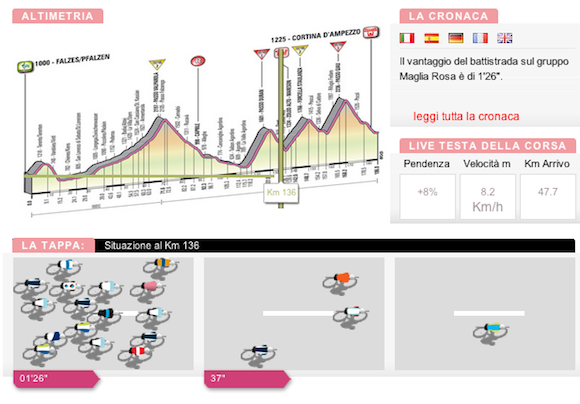
\includegraphics[scale=0.6]{05bericht/images/giro.png}
\end{figure} 

In der Abbildung \ref{fig:giro} ist der Live Abschnitt der offiziellen Webseite zu sehen. Im oberen Teil wird der Standort in der aktuelle Etappe eingeblendet. Unten ist die Situation an der Spitze abgebildet. Die Fahrer sind nach Rückstand gruppiert.
\\

Da jedoch nicht zu erkennen ist, wie die Informationen im Feld erfasst werden, muss die Mitbewerberanalyse an dieser Stelle abgeschlossen werden.
\chapter{Architektur}
Im folgenden Abschnitt wird die Architektur der Applikation diskutiert. Die Architektur ist so gewählt, dass die einzelnen funktionalen Komponenten zueinander eine tiefe Abhängigkeit aufweisen und dadurch eine weitere Entwicklung möglichst einfach ist.

\section{Struktur der Applikation}
%ja, plural ist Status, http://de.wikipedia.org/wiki/Status
Die Applikation hat im Grunde zwei Status, einerseits werden vor dem Rennen die Fahrerliste und die Marschtabelle importiert, andererseits wird die Rennsituation während dem Rennen erfasst und Änderungen festgehalten. Diese beiden Status können aber nicht absolut voneinander getrennt werden, da während dem Rennen Änderungen denkbar sind. Während dem Rennen müssen gewisse Daten immer angezeigt werden. Diese Live Informationen werden deshalb als eigene Ebene abgebildet. Aus den Anforderungen und den Kriterien entsteht folgende baumartige Struktur.

\begin{figure}[h!]
\caption{Struktur der Applikation als Organigramm}
\centering
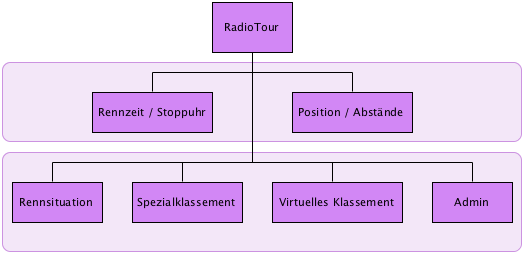
\includegraphics[scale=0.9]{05bericht/images/struktur.png}
\end{figure} 

Der Stamm stellt die Applikation dar und die Äste zeigen die Aufteilung der Funktionen. Die Rennzeit sowie die aktuelle Rennposition sind in einem immer sichtbaren Bereich platziert.
\\
Die untere Ebene beinhaltet die Kernelemente der Applikation. Diese werden in Views seitenweise dargestellt. Durch eine Navigation lässt sich zwischen den Views wechseln, ohne dass dabei die Live Informationen ausgeblendet werden.

\newpage

\section{Schichtenmodell und Paketdiagramm}
Die Applikation lässt sich in vier verschiedene Schichten aufteilen. Diese Schichten sind in der folgenden Grafik illustriert. Die oberste Schicht stellt dabei die Schnittstelle zum Benutzer dar. Innerhalb der Schicht werden die dabei verwendeten Pakete angezeigt.  
\begin{figure}[h!]
\caption{Die Schichten der Applikation inklusive der verwendeten Pakete}
\label{fig:layer}
\centering
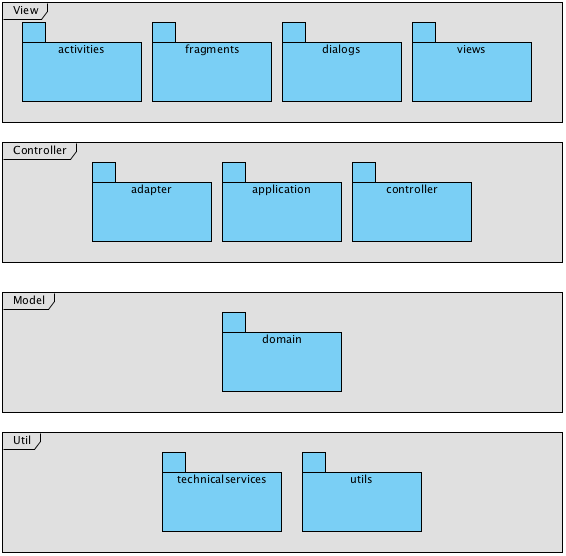
\includegraphics[scale=0.9]{05bericht/images/packagediagram.png}
\end{figure} 

Die \textit{View} Schicht in der Abbildung \ref{fig:layer} enthält alle Pakete in welchen Elemente zur Benutzerinteraktion definiert sind. Um die einzelnen Pakete in dieser Schicht zu verstehen, wird hier ein kurzer Exkurs zu Android View Elementen eingeschoben. Für die Elemente \textit{Activity} und \textit{Fragment} wird hierfür ein Teil der Android \gls{api} Beschreibung zitiert.

\begin{quote}
\textit{An Activity is an application component that provides a screen with which users can interact in order to do something, such as dial the phone, take a photo, send an email, or view a map. Each activity is given a window in which to draw its user interface. The window typically fills the screen, but may be smaller than the screen and float on top of other windows.}\footnote{Android Developers Reference, \url{http://developer.android.com/guide/topics/fundamentals/activities.html}, aufgerufen am 31.05.2012.}
\end{quote}

Die \textit{RadioTour} Applikation besteht aus einer Activity. Dies aus der Entscheidung heraus, dass gewisse Inhalte, wie zum Beispiel die aktuelle Etappe oder die Stoppuhr jederzeit verfügbar sein müssen. Diese Activity befindet sich im Paket \textit{activities}

\begin{quote}
\textit{A Fragment represents a behavior or a portion of user interface in an Activity. You can combine multiple fragments in a single activity to build a multi-pane UI and reuse a fragment in multiple activities. You can think of a fragment as a modular section of an activity, which has its own lifecycle, receives its own input events, and which you can add or remove while the activity is running (sort of like a "`sub activity"' that you can reuse in different activities).}\footnote{Android Developers Reference, \url{http://developer.android.com/guide/topics/fundamentals/fragments.html}, aufgerufen am 31.05.2012.}
\end{quote}

Eine spezielle Form der Fragmente stellen DialogFragmente dar. Sie werden benutzt um einen Dialog über der Activity einzublenden. In der Applikation werden diese Elemente verwendet um Daten zu erfassen und zu ändern. Die DialogFragmente der Applikation befinden sich im Paket \textit{dialogs}.

Für eine genauere Analyse der in der \textit{View} Schicht verwendeten Elemente und Klassen sei auf das Kapitel \ref{ref:realisierung} verwiesen.
\\
Die \textit{Controller} Schicht in der Abbildung \ref{fig:layer} ist für die Aufbereitung der Daten welche von der \textit{View} Schicht dargestellt wird verantwortlich.

Die \textit{Model} Schicht in der Abbildung \ref{fig:layer} stellt die Daten Objekte für die Applikation zur Verfügung. Eine Darstellung der in der \textit{RadioTour} App  verwendeten Domain Objekte ist in der Abbildung \ref{fig:domain} ersichtlich.

Die \textit{Util} Schicht in der Abbildung \ref{fig:layer} beinhaltet die Dienstobjekte für den Datenbank Zugriff sowie für die Kommunikation der Applikation mit dem cnlab Server. Im Paket \textit{utils} befinden sich allgemein gebrauchte Hilfsmethoden.


\section{Klassendiagramm}
Die Domainlogik beinhaltet die Kernelemente der Applikation. Einerseits sind dies die Rennfahrer, welche Informationen über sich festhalten, andererseits die Etappe mit den Informationen zur Strecke. Während dem Rennen werden die Fahrer in Gruppen unterteilt. Auch diese Gruppen sind in der Domain abgebildet. Das Klassendiagramm des Domain Package zeigt die wesentlichen Elemente.

\begin{figure}[h!]
\caption{Die Domainklassen in der Abhängigkeit}
\label{fig:domain}
\centering
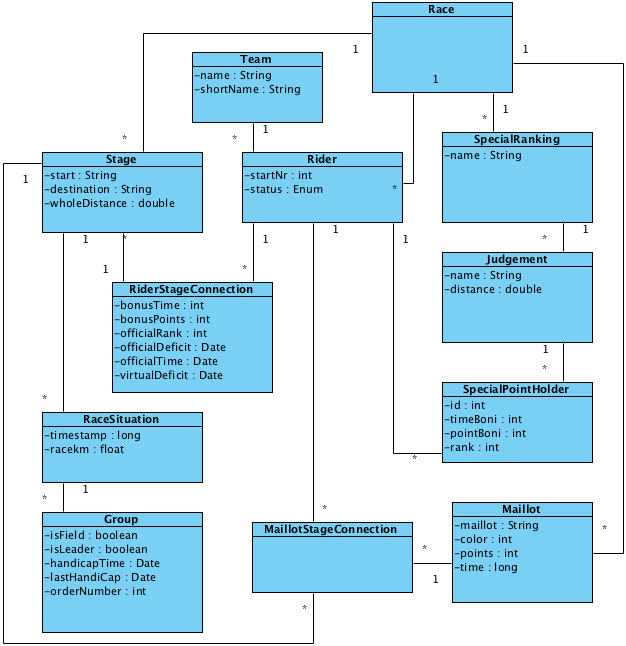
\includegraphics[scale=0.8]{05bericht/images/domain.png}
\end{figure} 


Die Klasse \textit{Rider} speichert die Angaben zu einem Fahrer und beinhaltet keine eigene Logik. Objekte dieser Klasse dienen als Stammdaten für alle Etappen welche in der Applikation erfasst sind.\\
Um die Fahrer nach Team sortiert anzeigen zu können, wird die Klasse \textit{Team} genutzt.\\
In \textit{Stage} ist die Etappe definiert. Jede Etappe hat eine Marschtabelle in Form von mehreren \textit{PointOfRace} Objekten. Diese Objekte werden durch Import der Marschtabelle erstellt.\\
Da pro Etappe jeder \textit{Rider} einen anderen \textit{RiderState} haben kann, gibt es die Verbindungsklasse \textit{RiderStageConnection}. In dieser Klasse ist jeweils die Etappe mit dem Fahrer verknüpft. Dies ermöglicht es, den Rückstand eines Fahrers in mehreren Etappen differenziert zu verfolgen. Dadurch werden bei einem Etappenwechsel innerhalb der Applikation immer die Informationen zur ausgewählten Etappe verwendet.\\
Die Klasse \textit{SpecialRanking} stellt ein Spezialklassement dar und wird benötigt, um die einzelnen Wertungen (\textit{Judgement}), welche Etappen basiert sind, auch über alle Etappen hinweg zu verrechnen. Damit können zum einen Punkte- bzw. Zeitboni pro Etappe verrechnet werden, was zur Darstellung im Virtuellen Klassement gebraucht wird und zum andern eine Rangliste pro Spezialklassement geführt werden. Diese Rangliste enthält die Ergebnisse aller Wertungen des angegebenen Spezialklassements ohne Rücksicht auf die zugehörige Etappe.\\
Die \textit{SpecialPointHolder} Klasse dient dazu, den zu Wertungen zugewiesenen Fahrern in der Datenbank zu speichern und zur späteren Berechnung des virtuellen Klassements berücksichtigen.\\
Eine \textit{RaceSituation} stellt einen Stand von \textit{Group} Objekten zu einem speziellen Zeitpunkt und Kilometerstand dar. Objekte vom Typ \textit{RaceSituation} werden bei jeder Neugruppierung von Fahrern oder Setzen eines Rückstandes einer Gruppe erstellt, an den Server gesendet und in die lokale \gls{sqlite} Datenbank geschrieben. Jeweils beim Start der Applikation sowie beim Wechseln der aktuellen Etappe wird die zuletzt in der Datenbank abgespeicherte \textit{RaceSituation} geladen. Die \textit{Group} Klasse enthält die Angaben zum aktuellen Rückstand zur Spitze, dem letzten bekannten Rückstand sowie boolsche Attribute welche bestimmen ob die Gruppe das Feld oder die Spitze darstellt.\\
Mit Hilfe der \textit{Maillot} Klasse können Maillots erstellt und verteilt werden, welche dann über alle Etappen bestehen. Da nach jeder Etappe ein anderer Fahrer ein Maillot tragen kann, wird eine Verbindung zwischen der Etappe und einem Maillot gebraucht. Diese Funktion wird durch die Klasse \textit{MaillotStageConnection} erfüllt. 

\newpage

\section{Datenbankschema}
Die Nutzung von ORMLite zur Objektrelationalen Abbildung von Instanzen in die \gls{sqlite} Datenbank impliziert, dass das Datenbankschema der Klassenstruktur wie in \ref{fig:domain} abgebildet entspricht. 

\section{Sequenz Diagramm}
Der häufigste UseCase besteht darin, die Rennsituation zu erfassen und an den Server zu übermitteln. Gleichzeitig werden im Hintergrund die Live Informationen aktualisiert. Diese beiden Hauptanwendungsfälle sind im folgenden System Sequenz Diagramm dargestellt. Der Actor wird durch den \textit{RadioTour Speaker} dargestellt und das System durch die \textit{RadioTour} Applikation. Das externe System stellt die Serverseite dar.

\begin{figure}[h!]
\caption{Das System Sequenz Diagramm}
\label{fig:ssd_rennen}
\centering
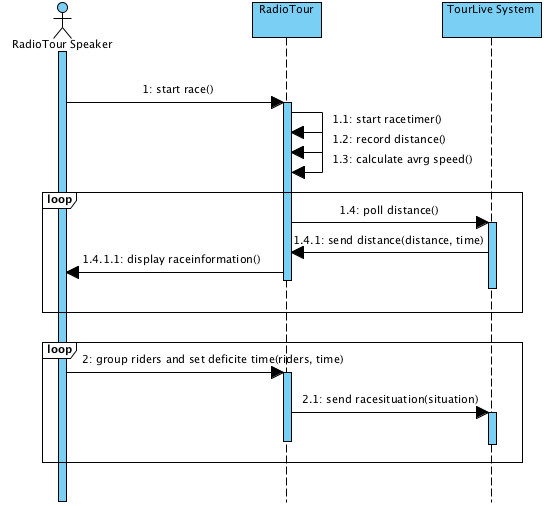
\includegraphics[scale=0.9]{05bericht/images/ssd_rennen.png}
\end{figure} 

Das Rennen wird durch das Starten der Rennzeit gestartet. Ab diesem Zeitpunkt beginnt die Aufzeichnung des Rennkilometers und die Berechnung der durchschnittlichen Geschwindigkeit.
\chapter{Realisierung}
\label{ref:realisierung}
\subsection{Externe Libraries}
\textbf{ORMLite (Version 4.39)}
Dieses Kapitel widmet sich der Realisierung der Applikation inklusive der grafischen Erscheinung. Zudem werden die wichtigsten Infos, um einem Entwickler beim Industriepartner einen schnellen Einstieg in das Weiterführen des Projektes zu ermöglichen, vermittelt.
 
Zur Speicherung der Objekte in die SQLite Datenbank des Tablet wird die Java Library ORMLite der Version 4.39 benutzt. In der Zwischenzeit sind neue Releases der Library auf der Webseite \url{http://ormlite.com/releases/} erschienen. Um sich in die Library einzulesen wird auf \url{http://ormlite.com/sqlite_java_android_orm.shtml} verwiesen.
\\
Um eine Änderung an den zu persistierenden Objekten durchzuführen ist es notwendig, die Klasse DatabaseConfigUtil.java im

\begin{lstlisting}{Name}
package ch.hsr.sa.radiotour.technicalservices.database;
\end{lstlisting}

als normale Java Applikation auszuführen. Dies generiert das \textit{Configuration File}

\textit{res/raw/ormlite\_config.txt}

welches für eine effizientere Ausführung von \textit{ORMLite} gebraucht wird.

\section{Aktuelle Erscheinung}
\subsection{Activity}

Die \textit{RadioTour} App besteht aus einer Activity wie in Abbildung \ref{gesamteactivity} dargestellt wird. Diese Activity wird in zwei Hauptteile eingeteilt. Es sind dies der (1)Header- sowie der (2)Hauptbereich. 

Activity:
\begin{lstlisting}{Name}
package ch.hsr.sa.radiotour.activities;
public class RadioTourActivity extends Activity 
	implements Observer, OnClickListener
\end{lstlisting}


View definiert in:
\textit{res/layout/base\_activity.xml}

Die \textit{RadioTourActivity} Klasse ist der Startpunkt der Applikationsausführung und deshalb im \textit{AndroidManifest.xml} File als Startactivity eingetragen. Das AndroiManifest.xml ist eine Datei welche in jedem Android Projekt im Stammverzeichnis vorhanden sein muss. Es enthält wichtige Informationen zur Applikation, unter anderem die Startactivity.


\begin{figure}[h!]
\caption{Gesamte Activity}
\label{fig:gesamteactivity}
\centering
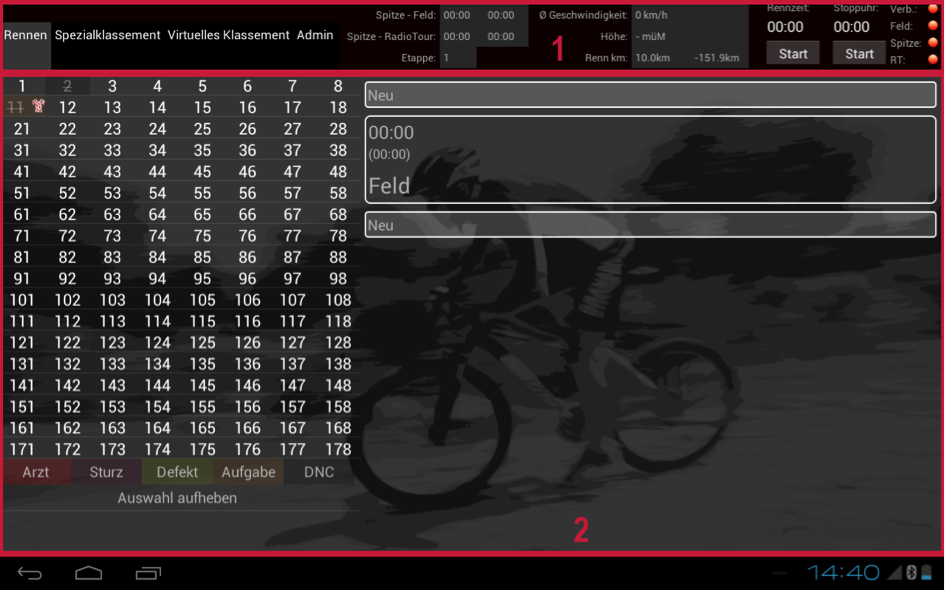
\includegraphics[scale=0.8]{07anhang/images/dev_activity.png}
\end{figure}

\subsection{Headerbereich}

\begin{figure}[h!]
\caption{Header Bereich}
\label{fig:headerbereich}
\centering
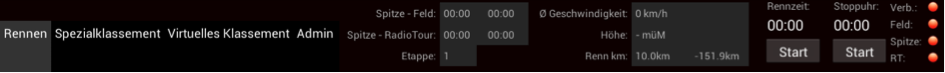
\includegraphics[scale=0.8]{07anhang/images/dev_header.png}
\end{figure}


\begin{lstlisting}{Name}
package ch.hsr.sa.radiotour.fragments;
public class HeaderFragment extends Fragment
	implements Observer, TimePickerIF
\end{lstlisting}

View definiert in:
\textit{res/layout/header\_fragment.xml}

Das \textit{HeaderFragment}, welches in Abbildung \ref{fig:headerbereich} illustriert ist, enthält alle Informationen, welche zu jedem Zeitpunkt der Applikationsausführung sichtbar sind. Dazu gehört der Systemzustand der zusätzlichen TourLive Komponenten welche via den TourLive Server über \gls{json} die \textit{RadioTour} Applikation mit Informationen versorgt.

Zudem werden wichtige Angaben zum derzeitigen Stand des Rennens im \textit{HeaderFragment} angezeigt, welche direkt aus der Tablet Anwendung stammen. Es sind dies die aktuelle Rennzeit und der aktuelle Rennkilometer, welcher, wie auch die aktuelle Höhe über Meer und die durchschnittliche Geschwindigkeit, aus dem im Tablet integrierten GPS Empfänger stammen. Um Fehlangaben zu korrigieren, ist die Kilometer- sowie die Rennzeitangabe editierbar.
Zeitabstände werden mit der ebenfalls im \textit{HeaderFragment} vorhandenen Stoppuhr gemessen. 
Mit einem Klick auf den "`Etappe"' Text wird die Marschtabelle, welche bereits absolvierte Stationen ausgraut, angezeigt.

\subsection{Hauptbereich}
Der Hauptbereich wird je nach ausgewähltem Tab (im Headerbereich) mit einem anderen Fragment ausgefüllt.
\\

\begin{figure}[h!]
\caption{RaceFragment}
\label{fig:racefragment}
\centering
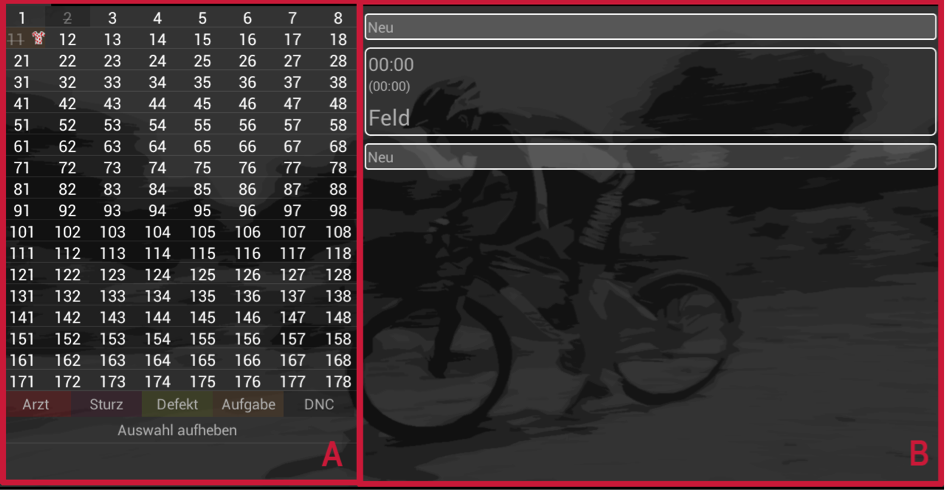
\includegraphics[scale=0.8]{07anhang/images/dev_racefragment.png}
\end{figure}


\textbf{RaceFragment.java}
\begin{lstlisting}{Name}
package ch.hsr.sa.radiotour.fragments;
public class RaceFragment extends Fragment 
\end{lstlisting}


View definiert in:
\textit{res/layout/race\_layout.xml}
\\
Das \textit{RaceFragment} welches in Abbildung \ref{fig:racefragment} zu sehen ist, beinhaltet zwei weitere Fragments. Das \textit{RaceFragment} an sich beinhaltet keine Funktionalität und dient nur zum Zusammenführen der zwei Fragmente \textit{DriverPickerFragment} und \textit{RiderGroupFragment}

\textbf{RiderPickerFragment}
\begin{lstlisting}{Name}
package ch.hsr.sa.radiotour.fragments;

public class RiderPickerFragment extends ListFragment
	implements OnClickListener
\end{lstlisting}

Das \textit{RiderPickerFragment}, Fragment A in Abbildung \ref{fig:racefragment} ermöglicht die Auswahl von einem oder mehreren Fahrern für die Zuweisung in eine Gruppe oder einem Spezialevent, siehe Abschnitt \ref{sec:requirements}. Die ausgewählten Fahrer können entweder per Drag and Drop oder mit anklicken des Zielfeldes zugewiesen werden. Mit einem Klick auf den "`Auswahl aufheben"' Text werden die bereits ausgewählten Fahrer wieder deselektiert.

Die Darstellung der Daten wird mithilfe eines \textit{ArrayAdapter<Team>} erzeugt. Dabei wird für jedes Team Objekt eine Zeile mit den jeweiligen Fahrern generiert. Die Textfelder mit den Spezialevents werden über eine dem \textit{RiderPickerFragment} hinzugefügten \textit{FooterView} ergänzt.

\textbf{RiderGroupFragment}
\begin{lstlisting}{Name}
package ch.hsr.sa.radiotour.fragments;

public class RiderPickerFragment extends Fragment
\end{lstlisting}


View definiert in:
\textit{res/layout/group\_fragment.xml}

Das \textit{RiderGroupFragment}, Fragment B in Abbildung \ref{fig:racefragment} stellt die aktuelle Rennsituation dar. Die schmaleren grauen Feldern dienen dazu, neue Gruppen zu erstellen. Wenn im \textit{RiderPickerFragment} Fahrer ausgewählt sind, können diese in die graue Fläche gezogen werden (Drag and Drop) oder auf die Fläche geklickt werden.
Den im transparenten Feld gruppierten Fahrer kann ein Rückstand relativ zur Spitze eingetragen werden. Dieser Rückstand wird den Fahrern welche dieser Gruppe angehören berechnet und im virtuellen Klassement berücksichtigt.
\\

\textbf{SpecialRankingFragment}
\begin{figure}[h!]
\caption{SpecialRankingFragment}
\label{fig:specialrankingfragment}
\centering
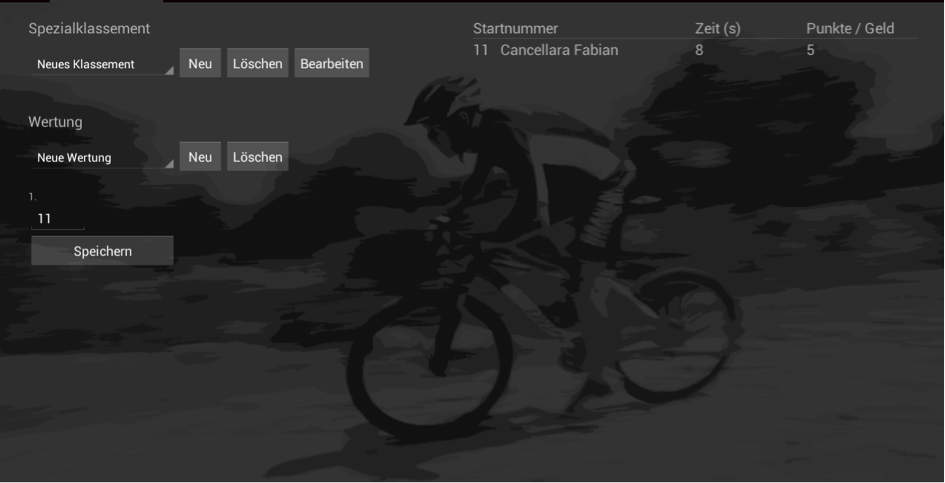
\includegraphics[scale=0.8]{07anhang/images/dev_specialranking.png}
\end{figure}


\begin{lstlisting}{Name}
package ch.hsr.sa.radiotour.fragments;

public class SpecialRankingFragment extends Fragment
\end{lstlisting}

View definiert in:
\textit{res/layout/special\_ranking\_fragment.xml}

Das \textit{SpecialRankingFragment}, abgebildet in Abbildung \ref{fig:specialrankingfragment}, erlaubt es neue Spezialklassemente und deren Wertungen, welche einer Etappe zugeordnet werden, zu erstellen. Eine Wertung beinhaltet Zeit- und/oder Punktebonus. Zudem kann jede Wertung eine unterschiedliche Anzahl berücksichtigte Anzahl Fahrer haben. Die Boni, welche Fahrer die in einer Wertung eine Klassierung erreichen, werden pro Spezialklassement rechts im \textit{SpecialRankingFragment} angezeigt. Die Etappenbasierte Verrechnung der Boni geschieht im \textit{VirtualRankingFragment}.




\textbf{VirtualRankingFragment}

\begin{figure}[h!]
\caption{VirtualRanking Fragment}
\label{fig:virtualrankingfragment}
\centering
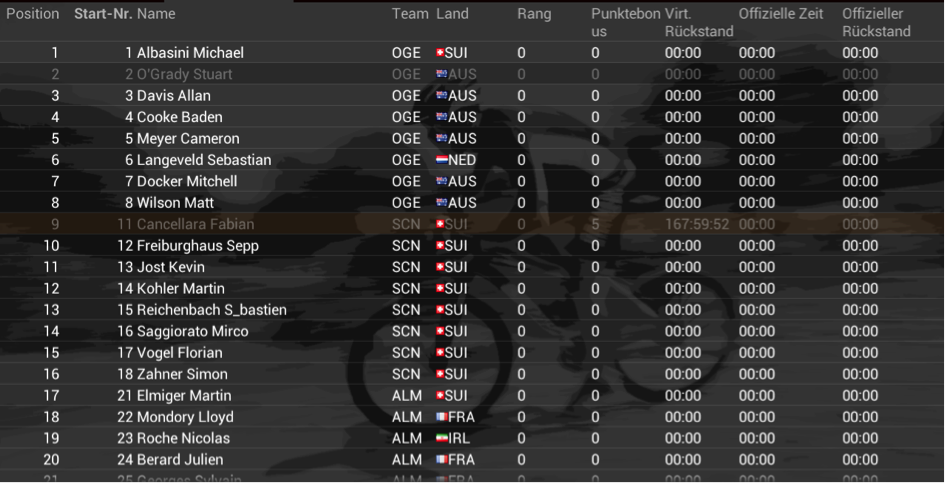
\includegraphics[scale=0.8]{07anhang/images/dev_virtual.png}
\end{figure}

\begin{lstlisting}{Name}
package ch.hsr.sa.radiotour.fragments;

public class VirtualRankingFragment extends ListFragment
\end{lstlisting}

Das \textit{VirtualRankingFragment} erbt von ListFragment und zeigt die zu der aktuell ausgewählten Etappe die dazugehörigen \textit{RiderStageConnection} (siehe Abbildung \ref{fig:domain}) an. Mit einem Klick auf einen Fahrer in der Rangliste lassen die Stammdaten des jeweiligen Fahrers verändern. So können zum Beispiel versehentlich als ausgeschieden markierte Fahrer wieder als im Rennen gesetzt werden. Über Klicks auf die  Spaltenbezeichnung lässt sich die Liste, sowohl auf- wie auch absteigend, nach den einzelnen Werten sortieren. Die Bezeichnung der aktuell sortierten Spalte wird fett dargestellt. Die Sortierung basiert auf der abstrakten \textit{RiderSortStrategy} Klasse, welche nach dem Vorbild des \textit{Strategy Pattern} implementiert wurde. 

\textbf{AdminFragment}

\begin{figure}[h!]
\caption{AdminFragment}
\label{fig:adminfragment}
\centering
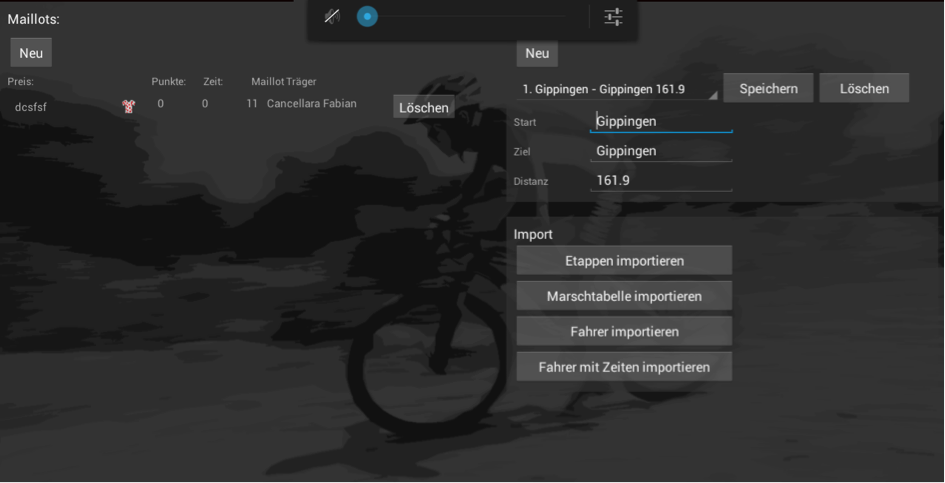
\includegraphics[scale=0.8]{07anhang/images/dev_adminfragment.png}
\end{figure}
\begin{lstlisting}{Name}
package ch.hsr.sa.radiotour.fragments;

public class AdminFragment extends Fragment
\end{lstlisting}


View definiert in:
\textit{res/layout/admin\_fragment.xml} 

\subsection{Offene Tasks}
Die Applikation ist weitgehend einsatzbereit. Folgende weitere Features sind noch offen:
\begin{itemize}
\item JSON
\item Importieren der Fahrerliste sowie der Etappeninformationen ist derzeit als .csv nur via USB möglich
\item Zeitabstände Feld-Spitze
\item Die Zeit- und Punkteboni der Maillots werden noch nicht im virtuellen Klassement verrechnet
\item Bei der Marschtabelle werden die abgefahrenen Stationen ausgegraut jedoch wird nicht auf die aktuelle Position „gescrollt“
\item Beim Wechsel einer Etappe wir die Rennzeit und der Rennkilometer nicht zurückgesetzt
\end{itemize}

\chapter{Testing}

\section{User Interface Tests}
Die Domain Klassen der RadioTour Applikation enthalten wenig bis gar keine Logik. Aus diesem Grund wird auf herkömmliche \glspl{junit} verzichtet. Als Ersatz dazu werden zwei Ansätze zum testen des User Interfaces verwendet. Zum einen ist ein Testprojekt mit Hilfe des Test Frameworks Robotium vorhanden. Anderseits wird der Android SDK interne Monkey verwendet.
\subsection{Robotium Testprojekt}
 Mit Hilfe von Robotium werden Klicks sowie Texteingaben an die Applikation gesendet. Das Testprojekt ist deshalb eine Form des automated User Interface Testings. Wird das Testprojekt gestartet führt es folgende Aufgaben durch:
\begin{itemize}
\item Starten der Applikation\\
Das Testprojekt startet die Applikation und wartet das erfolgreiche Ausblenden des Splashscreen ab
\item Importieren von Fahrern\\
Falls die Applikation keine Fahrerinformationen enthält,navigiert das Testprojekt mit Hilfe von gesendeten Klicks zum Admin Bereich der Applikation und wählt das richtige Import csv-File aus.
\item Gruppieren von Fahrern\\
Das Testprojekt wählt zwei Fahrer aus und setzt sie an die Spitze. Dabei wird getestet ob nach dem Auswählen wirklich zwei Fahrer ausgewählt sind und nach dem Gruppieren wieder keine.
\item Testen der Gruppen Konsistenz\\
Es wird getestet ob jeweils nur eine Gruppe mit der Bezeichnung "`Spitze"' sowie nur eine mit der Bezeichnung "`Feld"' vorhanden ist
\item Neustart der Applikation \\
Das Testprojekt schliesst die Applikation und startet sie neu. Dabei wird überprüft ob der Gruppenstand vor dem Schliessen der Applikation derjenigen nach dem Neustart entspricht
\item Neues Maillot erstellen\\
Mit Hilfe der gesendeten Klicks wird ein neues Maillot erstellt und ein Fahrer als Träger dieses Maillots eingestellt. Darauf wird überprüft ob zum angegeben Fahrer der Eintrag zum Maillot vorhanden ist.
\item Neues Spezialklassement erstellen\\
Das Testprojekt navigiert zum Spezialklassement Bereich und erstellt dort ein neues Spezialklassement sowie eine neue Wertung. Zu dieser Wertung werden die Gewinner eingegeben. Darauf wird überprüft ob die Bonuspunkte sowie Bonuszeit bei den angegebenen Fahrern korrekt eingetragen sind.
\item Löschen der oben erstellten Objekte \\
Die in den oben aufgeführten Aufgaben erstellten Objekte werden - bis auf die Fahrer -  gelöscht. Nach dem Löschen überprüft das Testprojekt ob sich alle Fahrer wieder in der Ausgangslage befinden.
 

\end{itemize}

\subsection{Android Monkey}
Der Android Monkey ist ein Kommandozeilentool welches auf jedem Android Gerät sowie dem Emulator ausgeführt werden kann. Das Tool sendet pseudo-zufällige Benutzer Events in schnellstmöglicher Abfolge an das System welches getestet wird. Dadurch werden Fehler im User Interface unabhängig von der darunter liegenden Logik aufgedeckt. Im Zusammenspiel mit dem Robotium Testprojekt kann deshalb, sofern beide Testmethoden erfolgreich durchlaufen, davon ausgegangen werden, dass die \textit{RadioTour} Applikation sich stabil und erwartungsgemäss verhält.

\section{Feldtest}

Um die Benutzerfreundlichkeit und den Mehrwert der Applikation im Vergleich zur bisherigen Web Applikation zu ermitteln ist ein Feldtest unabdingbar. Es gab die Möglichkeit die \textit{RadioTour} Applikation in einem Berner Fahrrad Rennen zu testen. Bei der Berner Rundfahrt\footnote{Berner Rundfahrt \url{http://www.berner-rundfahrt.ch}} bot sich der  \textit{RadioTour Speaker} der Berner Rundfahrt, David Loosli\footnote{David Loosli, ehemaliger profi Radrennfahrer und \textit{RadioTour Speaker} der Berner Rundfahrt} ,an die Applikation zu testen. In einem ersten Treffen wurden die grundlegenden Funktionen der Applikation und die Bedienung erklärt. Weiter ist ein Ausschnitt aus einem fiktiven Rennen durchgespielt worden, wobei eine Person den \gls{chronofunk} simulierte. Ein kurzer Auszug aus der vorbereiteten Situation ist unten aufgeführt.

\begin{itemize}
\item alle Fahrer sind importiert und das Rennen beginnt jetzt
\item Rennzeit wird gestartet
\item \textit{Chronofunk:} Fahrer 4 \& 17 von Beginn an, an der Spitze
\item \textit{Chronofunk:} Bereits 1:07 Vorsprung
\item \textit{Chronofunk:} 31 hat ein defektes Rad und muss raus
\item \textit{Chronofunk:} 8, 83 \& 34 fallen hinter das Feld mit einem Rückstand von 4:31
\end{itemize}

Der vollständige Usability Test sowie der Testlauf an der \textit{Berner Rundfahrt} mit den Rückmeldungen von Herrn Loosli sind im Anhang \ref{ref:usability} zu finden.

Mit den Erfahrungen und den Rückmeldungen aus diesem Event konnte das Endprodukt massiv verbessert werden. Die wesentlichen Punkte die für die Weiterentwicklung verwendet wurden sind:
\begin{itemize}
\item TimePicker Nummern (Auswahl des Rückstandes einer Gruppe) sind zu klein (Korrektur siehe Abbildung \ref{fig:timepicker})
\item nur die Fahrer welche aufgegeben haben oder nicht erschienen sind sollen ausgegraut werden (Vorschlag in Abbildung \ref{fig:riderpicker})
\item ein Fahrer kann folgende Status haben:
\begin{itemize}
\item im Rennen / aktiv
\item nicht gestartet
\item ausgeschieden
\end{itemize}
\item Rennzeit und Kilometer sind nach einem Absturz der Applikation noch verfügbar
\end{itemize}

\begin{figure}[h!]
\caption{TimePicker - Auswahl eines Zeitrückstandes}
\label{fig:timepicker}
\centering
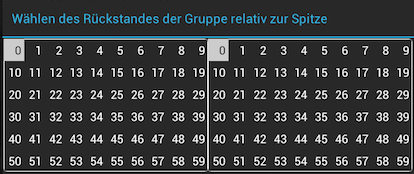
\includegraphics[scale=0.8]{05bericht/images/timepicker.png}
\end{figure} 
Besonders zu hervorheben ist an dieser Stelle, dass Herr Loosli entgegen den Erwartungen die Fahrer, welche in einer Gruppe eingeteilt sind (z.B. Spitze) nicht ausgegraut haben möchte. So entstand der, in Abbildung \ref{fig:riderpicker} dargestellte Entwurf.

\begin{figure}[h!]
\caption{RiderPicker - Auswahl von Fahrern}
\label{fig:riderpicker}
\centering
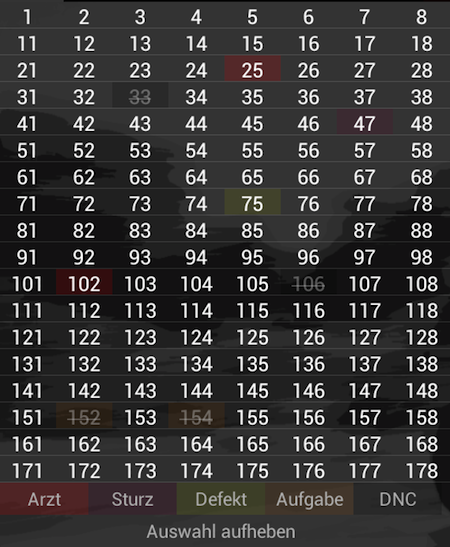
\includegraphics[scale=0.5]{05bericht/images/riderpicker.png}
\end{figure}

Die Abbildung \ref{fig:riderpicker} zeigt eine Situation, bei der die Fahrer 33 und 106 nicht gestartet sind und die Fahrer 152 und 154 aufgegeben haben. Diese Fahrer sind farblich markiert und durchgestrichen. Die weiteren Farben entsprechen den besonderen Ereignissen; Arzt, Sturz oder Defekt eines Fahrers bzw. eines Fahrrads.

\chapter{Ergebnisse und Schlussfolgerungen}
In diesem Kapitel werden die erreichten Ziele und das Endprodukt zusammengefasst und im Rahmen der Aufgabenstellung beurteilt. Des weiteren wird die Zukunft des Produktes und die weitere Entwicklung erörtert.

\section{Endprodukt}
Das Ziel war es, eine verbesserte und modernisierte Applikation für den \textit{RadioTour Speaker} zu erstellen, welche die bisherige Web Applikation ersetzt. Die Anforderungen bestanden aus den Features der bestehenden Lösung und wurden weitgehend erreicht. Zudem wurden die Wünsche und Anregungen des \textit{RadioTour Speakers} implementiert. Das Endprodukt beinhaltet die Android Applikation \textit{RadioTour} mit der passenden Hardware, einem Samsung Galaxy Tab 10.1. Diese Lösung ist im heutigen Stand, für die Begleitung von  Radrennen, einsatzfähig. Dies konnte durch den Einsatz an der Berner Rundfahrt bestätigt werden. Für die Entwicklung von weiteren Features und der Vorbereitung für die Verwendung an der Tour de Suisse wird die Applikation dem Industriepartner, der cnlab AG, übergeben.
\\

Gegen Ende des Projekts kamen noch weitere Anforderungen hinzu. 
So z.B. der Import der Fahrer direkt vom Server via \gls{json} oder das automatische Navigieren zur aktuellen Rennposition in der Marschtabelle. Da diese Anforderungen erst bei einem fortgeschrittenen Stadium des Projekts hinzukamen, konnten diese Features nicht mehr implementiert werden. Es handelt sich bei diesen Anforderungen nicht um kritische Bereiche, daher sind die Änderungen auch in Form eines Updates noch möglich.

\section{Ausblick}
Der nächste und letzte Feldtest der Applikation vor der Tour de Suisse erfolgt an den Radsporttage in Gippingen\footnote{Radsporttage Gippingen, \url{http://www.gippingen.ch/}, Aufgerufen am 30.05.2012.}. Da dieser Feldtest erst nach der Projektabgabe stattfindet, liegt er in der Obhut der cnlab AG. Das Feedback aus diesem Test wird zeigen, wie gut die Rückmeldungen aus der Berner Rundfahrt umgesetzt werden konnten.
\\

Bis zur Tour de Suisse gibt es also noch die Möglichkeit, Anpassungen vorzunehmen. Nach der Tour de Suisse, dem ersten Einsatz in einem Etappenrennen, ist eine weitere Auswertung und allfällige Optimierung sinnvoll. Mit dieser Arbeit wurde ein wichtiger Grundstein gelegt, mit dem weiter gearbeitet werden kann.


\listoffigures
\printglossary[style=altlist,title=Glossar]


\nocite{*}
\bibliographystyle {unsrt}
\bibliography{06verzeichnisse/02literaturverzeichnis}

\part{Anhang}

\section{BigPicture}
\label{fig:bigpicture}
Das Aufgabenumfeld in einem BigPicture zusammengefasst.
\begin{figure}
\includegraphics[scale=0.8]{07anhang/images/bigpicture.png}
\caption{Das BigPicture in voller Grösse}
\end{figure}

\section{Projektmanagement}

\section{Software Dokumente}

\section{Kriterienkatalog}
\label{ref_kriterien}
Hier sind die Kriterien

\section{Kaufempfehlung}
\label{ref_kaufempfehlung}

\section{UseCases der bisherigen Applikation}
\label{ref:usecases}
Im unten stehenden UseCase Diagramm (Abbildung \ref{fig:usecasediagram}) sind die primären UseCases aufgeführt. Nur der RadioTour Speaker erfasst Daten in dieser Applikation und ist daher der einzige Aktor. Das System wird durch die RadioTour Applikation abgebildet. Zur besseren Darstellung wurden einzelne UseCases vereinfacht oder zusammen gefasst.
\begin{figure}[h1]
  \caption{UseCase Diagramm}
  \label{fig:usecasediagram}
  \begin{center}
    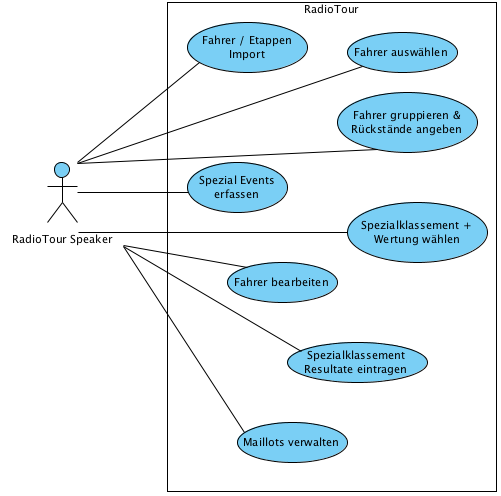
\includegraphics[scale=0.6]{05bericht/images/usecasediagram.png}
  \end{center}
\end{figure}

\begin{itemize}
\item \textbf{Fahrer auswählen}\\
Dem RadioTour Speaker muss es möglich sein, einen oder mehrere Fahrer schnell auszuwählen. Die Fahrer werden im Auswahldialog bevorzugt durch ihre Startnummern dargestellt. An der Tour de Suisse besteht ein Team – nach Aussage von P. Heinzmann – aus 8 Fahrern. Um eine möglichst gute Übersicht zu gewährleisten werden die Fahrer jeweils Zeilenweise in deren Teams gruppiert. Ausgewählte Fahrer werden farblich hervorgehoben. Die Nummern der Fahrer, welche bereits Gruppen zugewiesen wurden, werden in Klammern dargestellt. Die Nummern ausgeschiedener Fahrer werden gestrichen dargestellt.

\begin{figure}[h!]
  \caption{Die Fahrerauswahlliste zur Gruppierung in der bisherigen Web Applikation}
  \begin{center}
    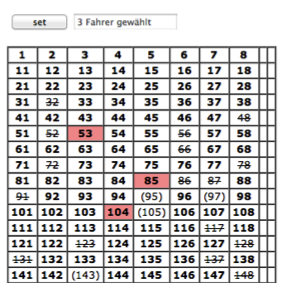
\includegraphics{05bericht/images/uc01_fahrerliste.png}
  \end{center}
\end{figure}

\item \textbf{Fahrer gruppieren}\\
Dem RadioTour Speaker muss es möglich sein, die ausgewählten Fahrer in Gruppen zu organisieren. So kann er die ihm gemeldeten Rennsituationen mit Ausreissern, Verfolgern, Feld und abgehängten darstellen.

\begin{figure}[H]
  \caption{Gruppierung in der bisherigen Web Applikation}
  \begin{center}
    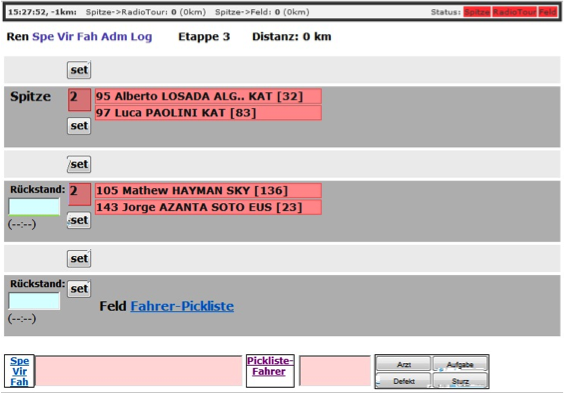
\includegraphics{05bericht/images/uc02_gruppen.png}
  \end{center}
\end{figure}

\item \textbf{Rückstände angeben}\\
Dem RadioTour Speaker muss es möglich sein, für die Gruppen (siehe oben) ihre jeweiligen Zeitabstände relativ zur Spitze einzugeben. Falls vorhanden, sollen auch die mit dem TourLive GPS-System erfassten Zeitabstände Spitze-Feld eingeblendet werden.

\item \textbf{Spezial Events erfassen}\\
Dem RadioTour Speaker muss es möglich sein, für ausgewählte Fahrer Spezialereignisse festzulegen. Dies sind beispielsweise Arztbesuch, Aufgabe, Defekt oder einen Sturz.
\begin{figure}[H]
  \caption{Die Spezialklassemente und Wertungen in der bisherigen Web Applikation}
  \begin{center}
    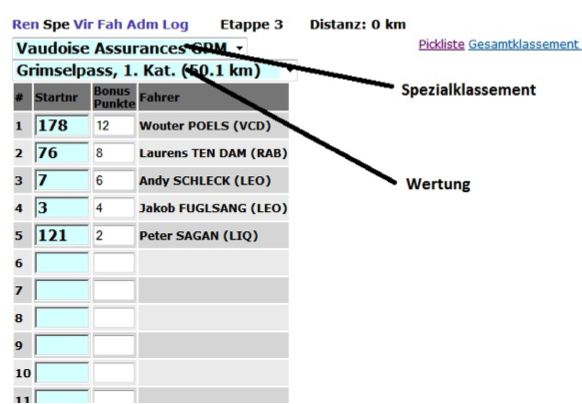
\includegraphics{05bericht/images/uc03_spezial.png}
  \end{center}
\end{figure}


\item \textbf{Spezialklassement und Wertung wählen}\\
Bei Mehretappenrennen werden typisch neben dem Gesamtklassement (schnellster Fahrer) mehrere Spezialklassemente (z.B. Bergpreis-, Sprintwertung, Punkteklassement) gewertet. Innerhalb der Etappen gibt es jeweils mehrere Stellen (Wertungen), an denen für die Spezialklassemente Punkte vergeben werden. Dem RadioTour Speaker muss es möglich sein, die gewünschte Wertung zu einem der vorher erfassten Spezialklassemente auszuwählen.

\item \textbf{Spezialklassement Resultate eintragen}\\
Dem RadioTour Speaker muss es möglich sein, für eine Wertung welche er ausgewählt hat (siehe UC oben), die Ränge zur Wertung mit Fahrernummern zu verbinden, wodurch das Klassement generiert wird.

\item \textbf{Klassement anzeigen}\\
Das durch die eingetragene Wertung erstellte Klassement muss vom RadioTour Speaker abgerufen werden können. Dort sollen alle Fahrer angezeigt werden, welche einen Punkterang in diesem Spezialklassement erreichten.

\item \textbf{Virtuelles Klassement}\\
Dem RadioTour Speaker muss es möglich sein, ein aktuelles Klassement der Tour abzurufen und dieses nach bestimmten Kriterien zu sortieren. Die zurzeit möglichen Sortierkriterien sind:
\begin{itemize}
\item[-]Gruppen (zur Zeit des Aufrufs, nicht offiziell)
\item[-]Virtueller Rückstand (zur Zeit des Aufrufs, nicht offiziell)
\item[-]Zeitboni (zur Zeit des Aufrufs, nicht offiziell)
\item[-]Offizielle Zeit (zum Etappenende des Vortages, offiziell)
\item[-]Offizieller Rückstand (zum Etappenende des Vortages, offiziell)
\end{itemize}

\begin{figure}[h!]
  \caption{Virtuelles Klassement in der bisherigen Applikation}

  \begin{center}
    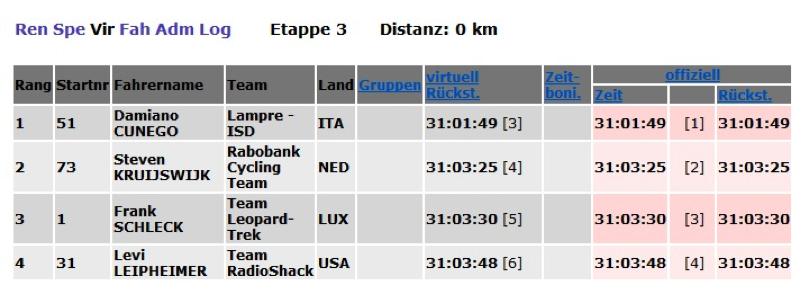
\includegraphics{05bericht/images/uc05_virtuell.png}
  \end{center}
\end{figure}

\item \textbf{Fahrerliste anschauen}\\
Dem RadioTour Speaker muss es möglich sein, die aktuelle Fahrerliste anzuschauen. Die Fahrerliste ist nach Startnummer aufsteigend sortiert. (Die Startnummern werden in Mehretappenrennen so vergeben, dass die Fahrer eines Teams aufeinanderfolgende Startnummern erhalten.)

\begin{figure}[h!]
  \caption{Die Fahrerliste mit den Informationen zum Status der Fahrer}
  \begin{center}
    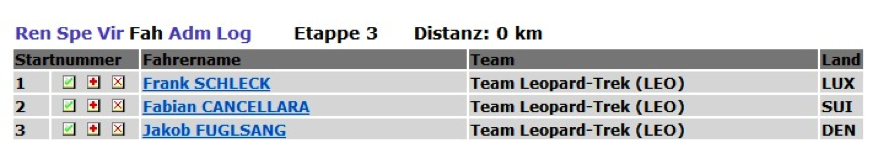
\includegraphics{05bericht/images/uc06_fahrerliste.png}
  \end{center}
\end{figure}

\item \textbf{Fahrer de- bzw. aktivieren}\\
Dem RadioTour Speaker muss es möglich sein, einzelne Fahrer zu deaktivieren bzw. wieder zu aktivieren. Der Grund der Deaktivierung soll auch später noch nachvollziehbar sein. Es soll möglich sein, den Grund für die Deaktivierung anzugeben (z.B. ausgeschieden, nicht gestartet, andere). 
Eine so vorgenommene Deaktivierung eines Fahrers muss durch den RadioTour Speaker Rückgängig gemacht werden können.

\item \textbf{Fahrerdetails bearbeiten}\\
Dem RadioTour Speaker muss es möglich sein, einen Fahrer aus der Fahrerliste auszuwählen um seine Details anzuschauen und auch zu bearbeiten. 

\item \textbf{Statistik}\\
Dem RadioTour Speaker muss es möglich sein, in seinem Admin-Bereich eine kurze und prägnante textbasierte Statistik zu erhalten, bei welcher er auf einen Blick sieht wie viele Fahrer in der Datenbank sind und welche davon aktiv sind. Darüber hinaus die Anzahl Gruppen, Spezialklassemente, Wertungen und Vergebene Punkte.

\item \textbf{Import Fahrerliste}\\
Nach jedem Renntag ( = Etappe), wird in die RadioTour Applikation eine neue Fahrerliste mit den aktuellen offiziellen Zeiten importiert. Die Herausforderung besteht darin, dass das Format dieser Fahrerlisten im vornherein nicht bekannt ist. Deshalb muss es dem RadioTour Speaker möglich sein, den Importmodus noch dynamisch anzupassen. Derzeit sind für den Import der Daten verschiedene Importverfahren implementiert wie im Screenshot ersichtlich ist.

\item \textbf{Import Spezialklassemente}\\
Dem RadioTour Speaker muss es möglich sein, Spezialklassemente zu importieren. Diese Importe werden vor der Tour de Suisse getätigt weshalb ein dynamischer Import hier nicht zwingend notwendig ist.

\item \textbf{Speicherung Maillots}\\
Dem RadioTour Speaker muss es möglich sein, die Belegung der 4 verschiedenen Maillots anzugeben und zu sichern. Folgende Maillots gibt es:

\begin{center}
  \begin{tabular}{ l | l  }
    \hline
    Name & Farbe \\ \hline
    \hline
    Bergpreis & Rot-Weiss \\ \hline
    Gesamtklassement & Gelb \\ \hline
    Neo-Profi & Weiss \\ \hline
    Punkte & Grün\\

    \hline
  \end{tabular}
\end{center}


\item \textbf{Daten exportieren}\\
Dem RadioTour Speaker muss es möglich sein, die Spezialklassemente, Wertungen, Fahrer nicht nur zu erfassen, importieren und bearbeiten, sondern auch als *.csv zu exportieren. Dabei werden einfach alle mit dem gewünschten Export assoziierten Infos in das exportierte *.csv geschrieben.

\end{itemize}




\end{document}	
